\subsection{Basic Idea}   \label{subsec:lossy_intro}

For real–valued sources perfect reconstruction with a finite number of
bits is impossible.  
A lossy code trades rate \(R\) (bits/symbol) for fidelity measured by
a single–letter distortion function \(d(x,\widehat x)\).
For mean–squared error (MSE) distortion
\[
D=\mathbb{E}\bigl[(X-\widehat{X})^2\bigr].
\]
Rate–distortion theory characterizes
\[
R(D)=\inf\{R:(R,D)\text{ achievable}\},\quad
D(R)=\inf\{D:(R,D)\text{ achievable}\}.
\]

\begin{example}[finite–precision \(\pi\)]
Approximating
\(\pi=3.1415926\ldots\) by  
\(\widehat\pi_1=3.14\) (rate \(=7\) bits, absolute distortion \(\approx10^{-3}\))  
vs.\ \(\widehat\pi_2=3.14159\) (rate \(=17\) bits, distortion
\(\approx2.65\times10^{-6}\)).
\end{example}

%%%%%%%%%%%%%%%%%%%%%%%%%%%%%%%%%%%%%%%%%%%%%%%%%%%%%%%%%%%%%%%%%%%%%%%%
\subsection{Scalar Quantization}              \label{subsec:scalar_quant}

Let us consider the height of $10,000$ people following a normal distribution with a mean of $170$ and a variance of $10$. We want to store the height of a specific person.

\paragraph{Rate \(R=0\).}
Outputting the constant \(\widehat{X}=\mathbb{E}[X]=170\) gives
\(D(0)=\operatorname{Var}(X)=10\).

\paragraph{Rate \(R=1\).}
Encoder
\(
e(x)=\mathbf 1\{x>170\}.
\)
Decoder chooses the conditional means
\[
d(0)=\mathbb{E}[X\,|\,X\leq170],\quad
d(1)=\mathbb{E}[X\,|\,X>170].
\]
For a normal distribution, $$\mathbb{E}[X|X\leq a]=\mu+\sigma\mathbb{E}[Z|Z\leq k],\quad k=\frac{a-\mu}{\sigma},$$
$$\mathbb{E}[Z|Z\leq k] = \frac{\int_{-\infty}^kz\phi(z)dz}{\Phi(k)}=-\frac{\phi(z)}{\Phi(z)},$$
where $\phi(\cdot)$ denotes the pdf of the normal distribution and $
\Phi(\cdot)$ denotes the cdf of it. Then the resulting distortion is
\(
D(1)=10\bigl(1-\tfrac2\pi\bigr)\approx3.64.
\) (check yourself!)

\paragraph{Rate \(R=2\).}
Thresholds \(165,170,175\) (four cells) give distortion $\approx 1.75$. However, there is no guarantee that this distortion is optimal.

%%%%%%%%%%%%%%%%%%%%%%%%%%%%%%%%%%%%%%%%%%%%%%%%%%%%%%%%%%%%%%%%%%%%%%%%
\subsection{Lloyd–Max Algorithm} \label{subsec:LM}

With fixed thresholds, differentiating
\(
D(R)=\sum_{i}\int_{\tau_i}^{\tau_{i+1}}f_X(x)(x-\widehat{x}_i)^2dx
\)
w.r.t.\ \(\widehat{x}_i\) yields
\(\widehat{x}_i=\mathbb{E}[X\mid \tau_i\le X<\tau_{i+1}]\).
With fixed \(\widehat{x}_i\) the derivative of \(D\) w.r.t.\ \(\tau_{i+1}\)
vanishes at
\(\tau_{i+1}=\tfrac12(\widehat{x}_i+\widehat{x}_{i+1})\).
Iterating these two steps decreases \(D\) monotonically and converges
to a local optimum. For the above example, we get $D(2)\approx 1.17.$

\begin{figure}[ht]
\centering
    \begin{subfigure}{0.40\textwidth}
        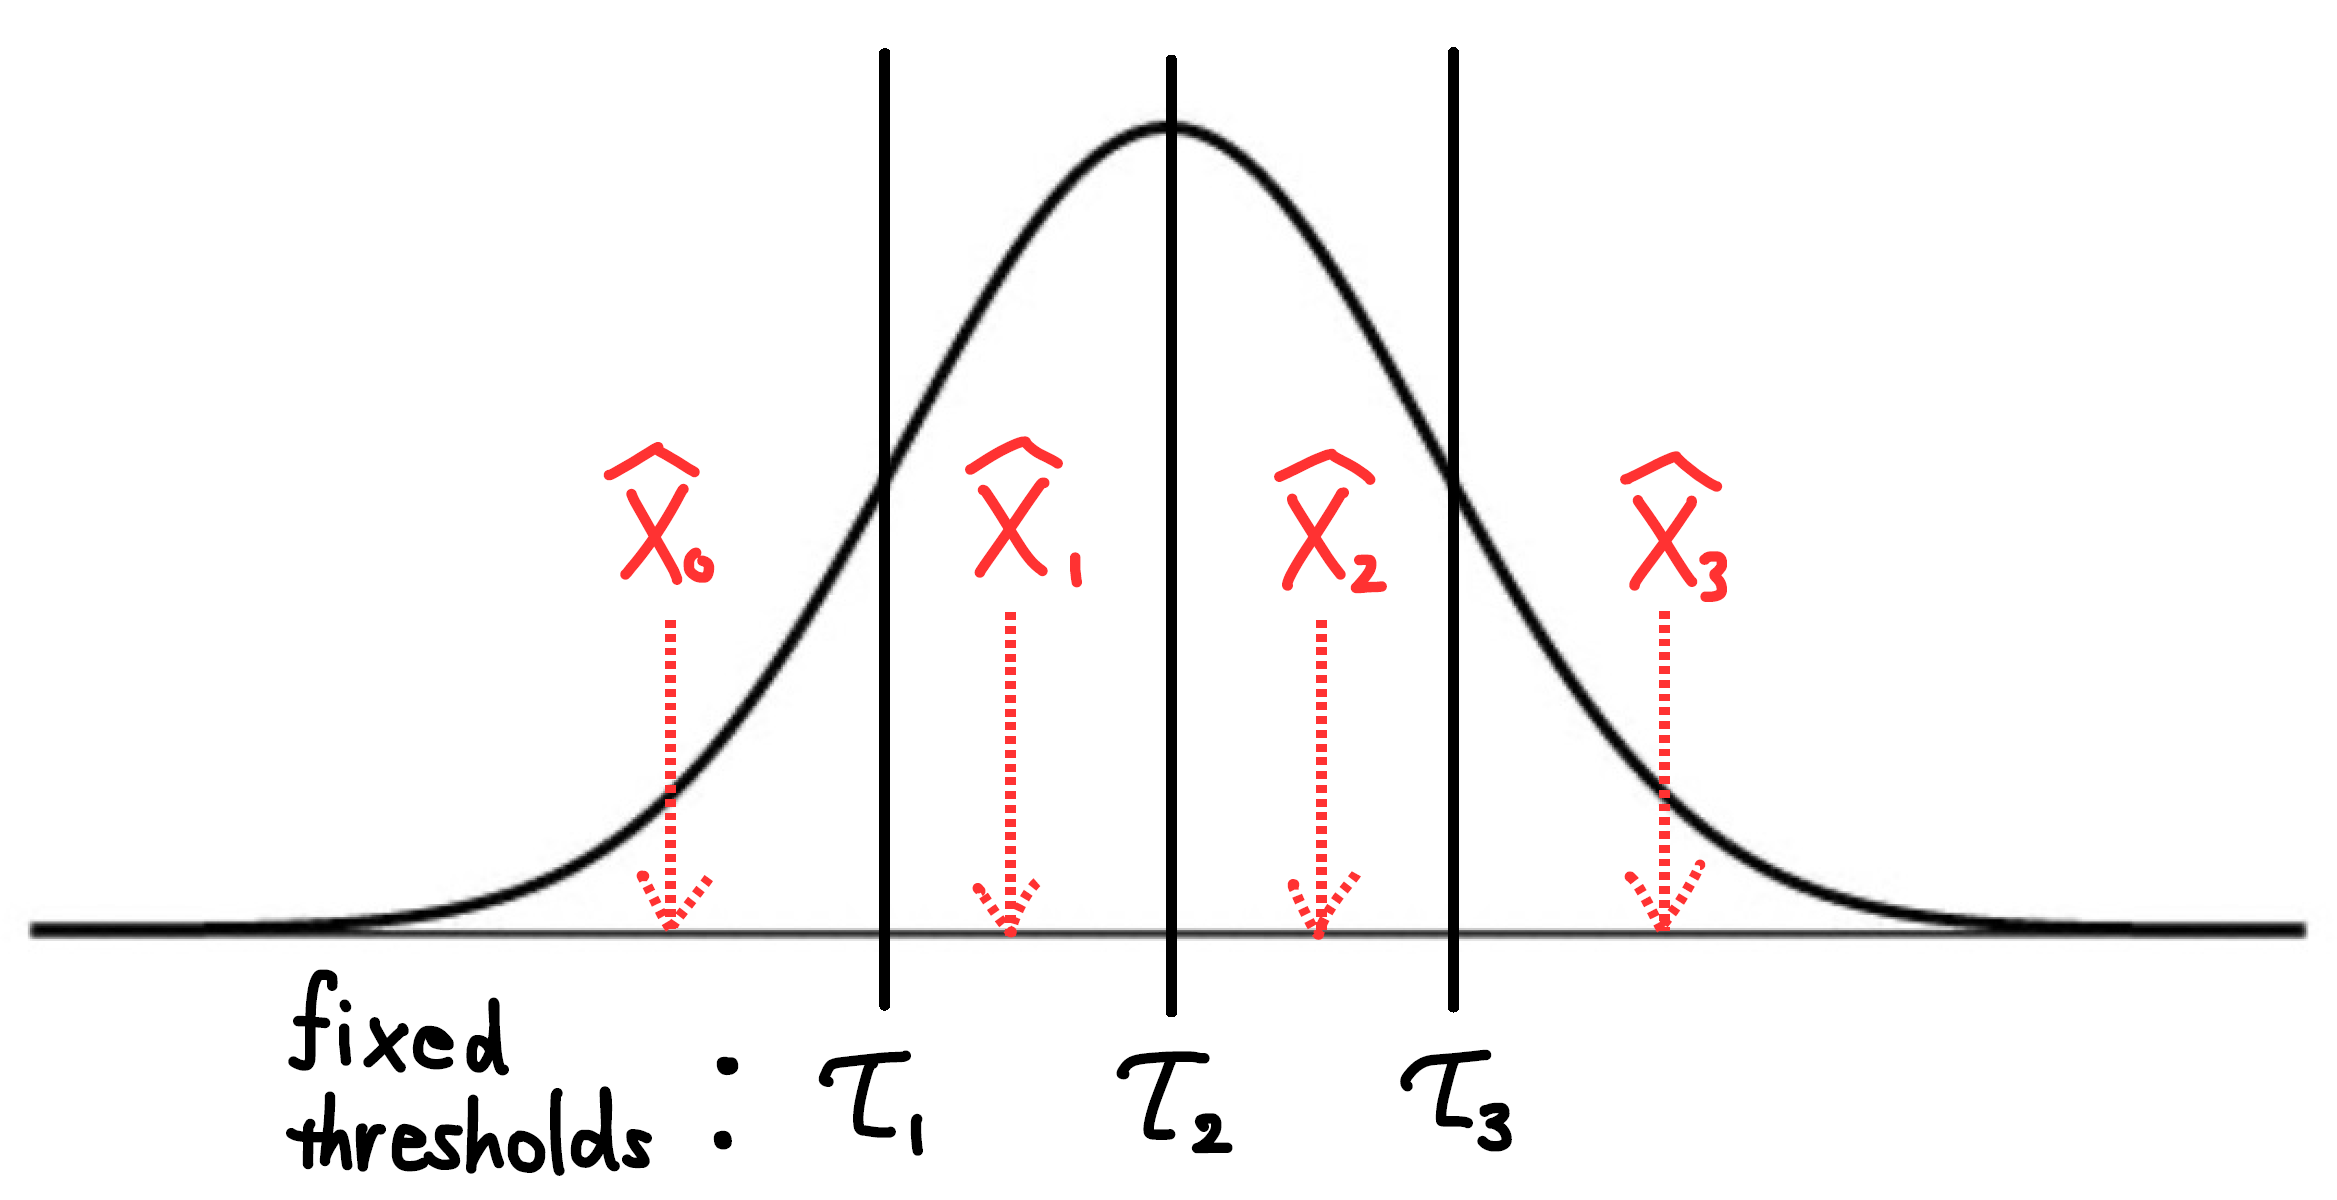
\includegraphics[width=\linewidth]{images/scribe19_image2a.png}
        \caption{Use fixed $\tau_i$'s to estimate $\widehat{X}_i$'s}
        \label{fig2a}
    \end{subfigure}
    \hfill
    \begin{subfigure}[b]{0.1\textwidth}
        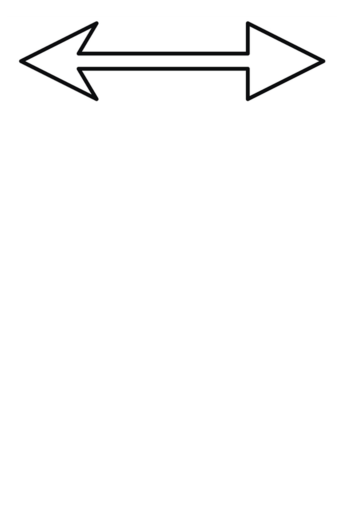
\includegraphics[width=\linewidth]{images/scribe19_arrow_both_directions.png}
    \end{subfigure}
    \hfill
    \begin{subfigure}[b]{0.40\textwidth}
        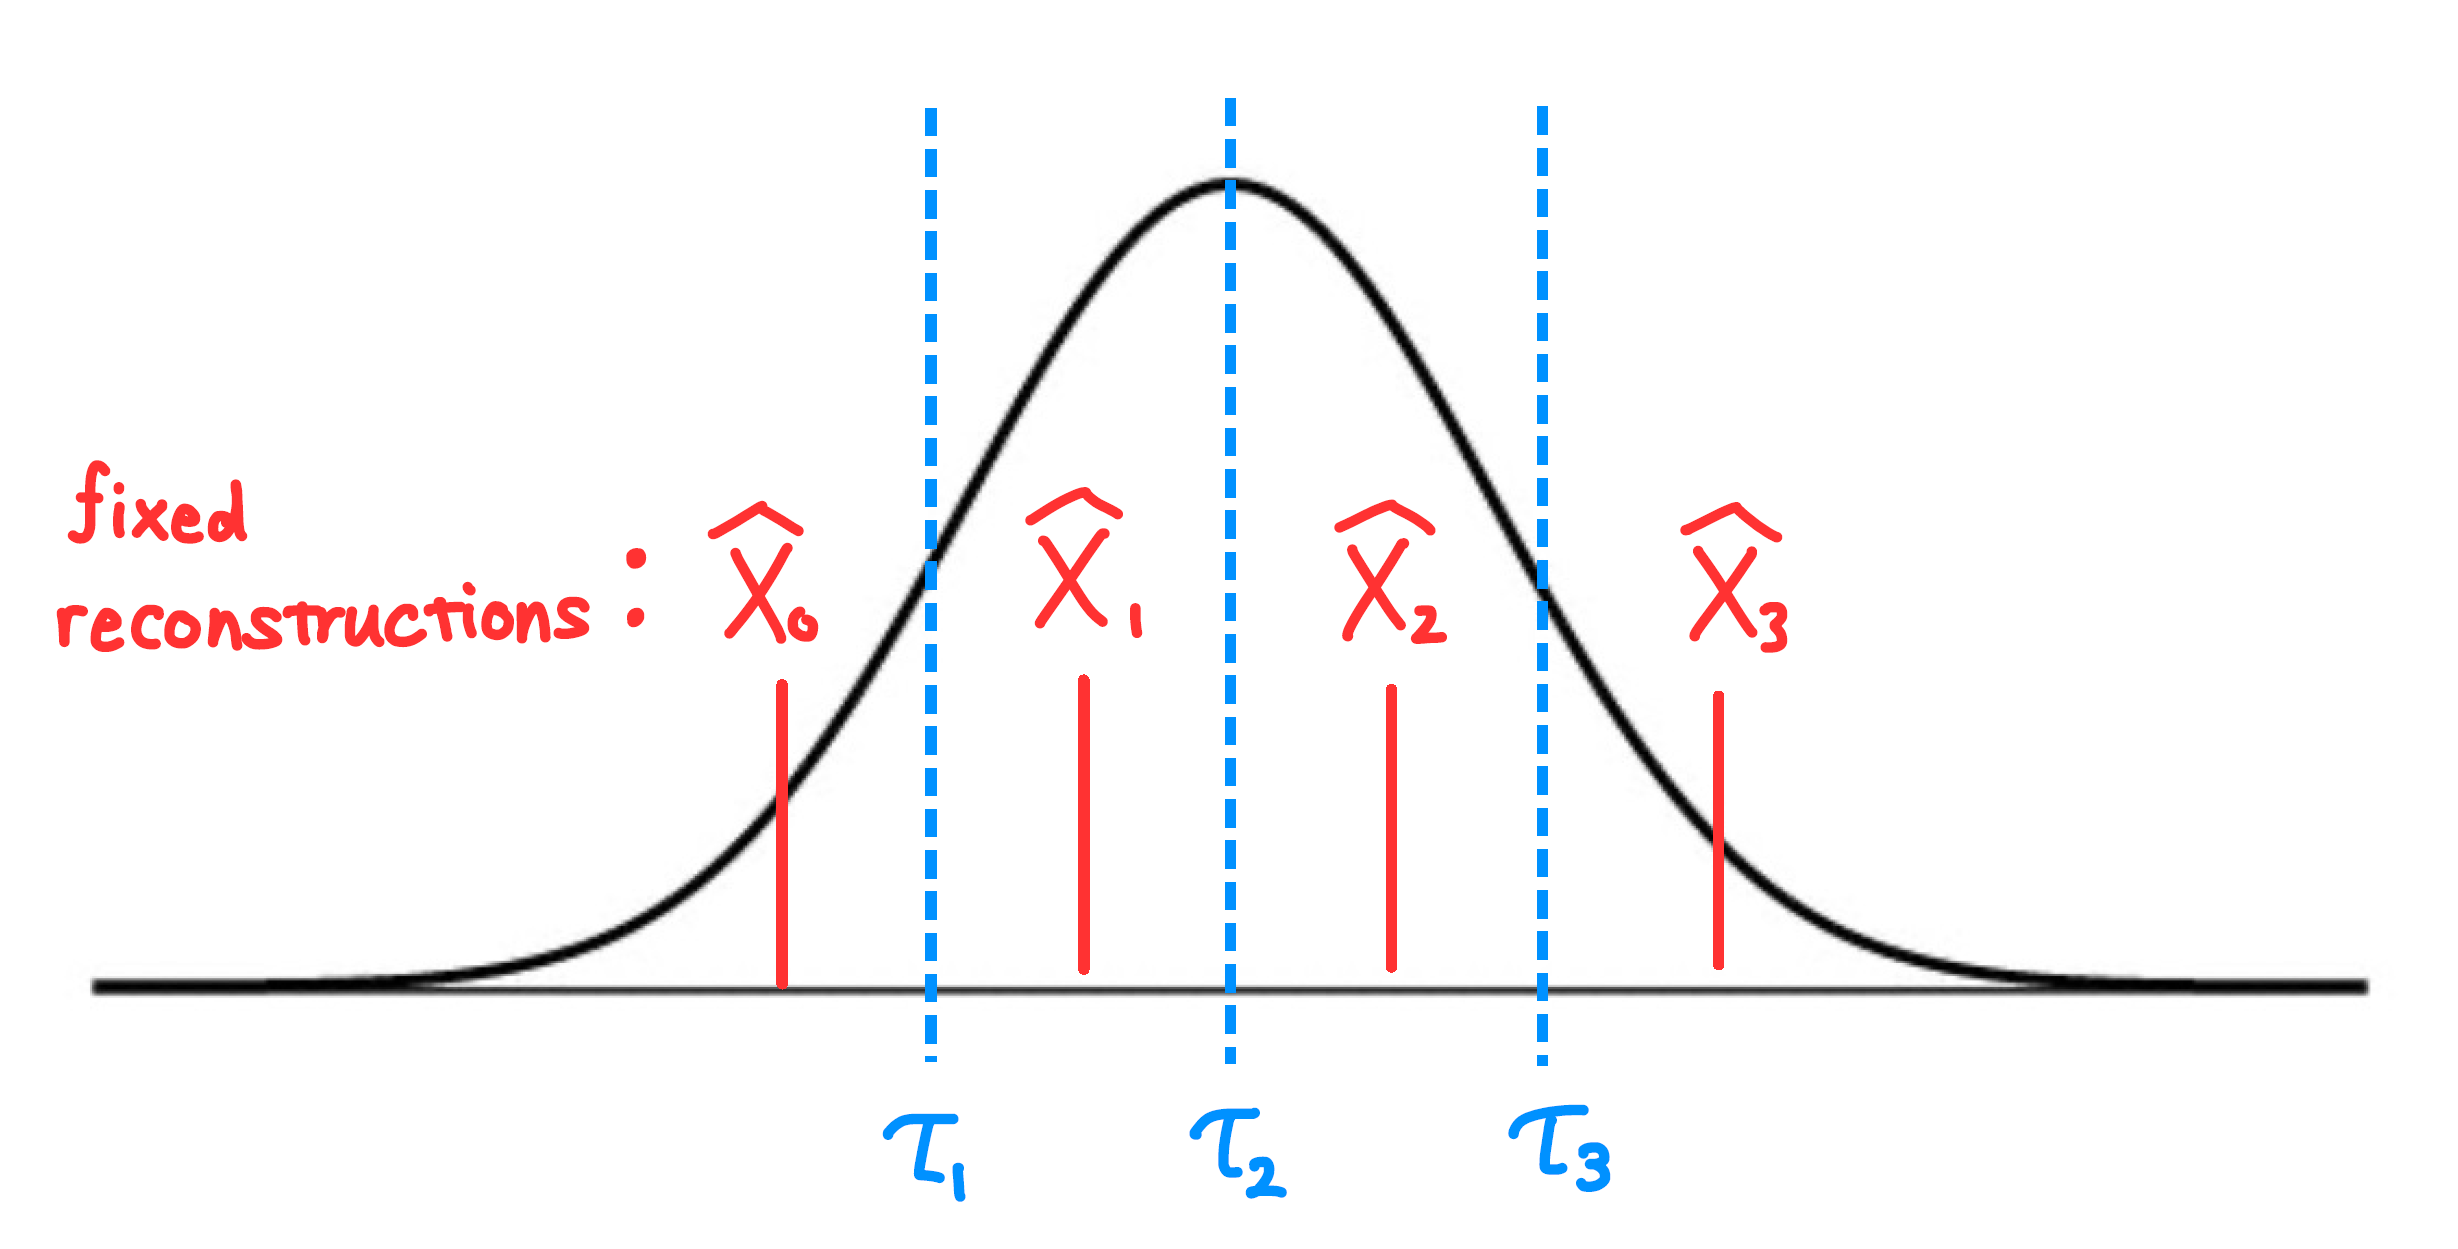
\includegraphics[width=\linewidth]{images/scribe19_image2b.png}
        \caption{Use fixed $\widehat{X}_i$'s to estimate $\tau_i$'s}
        \label{fig2b}
    \end{subfigure}
\caption{Alternating optimization of the thresholds and the representatives}
\label{fig2}
\end{figure}

%%%%%%%%%%%%%%%%%%%%%%%%%%%%%%%%%%%%%%%%%%%%%%%%%%%%%%%%%%%%%%%%%%%%%%%%
\subsection{Vector Quantization}\label{sec:vector_quantization}

Scalar quantization maps a one-dimensional continuous variable to  
\(M = 2^{R}\) reconstruction levels using a quantizer  
\[
  Q : \R \longrightarrow \{0,1,\dots,M-1\},
\]  
so that each symbol is represented with \(R\) bits.  
In \(n\)-dimensions we generalise to  
\[
  Q^{(n)} : \R^{n} \longrightarrow \{0,1,\dots,M-1\}, 
  \qquad M = 2^{nR},
\]  
which is called \emph{vector quantization (VQ)}.  
The examples below illustrate the difference.

\begin{example}
Let \((X_1,X_2)\) be independent and uniformly distributed on \([-1,1]^2\) (Figure~\ref{fig3}).

\begin{figure}[ht]
  \centering
  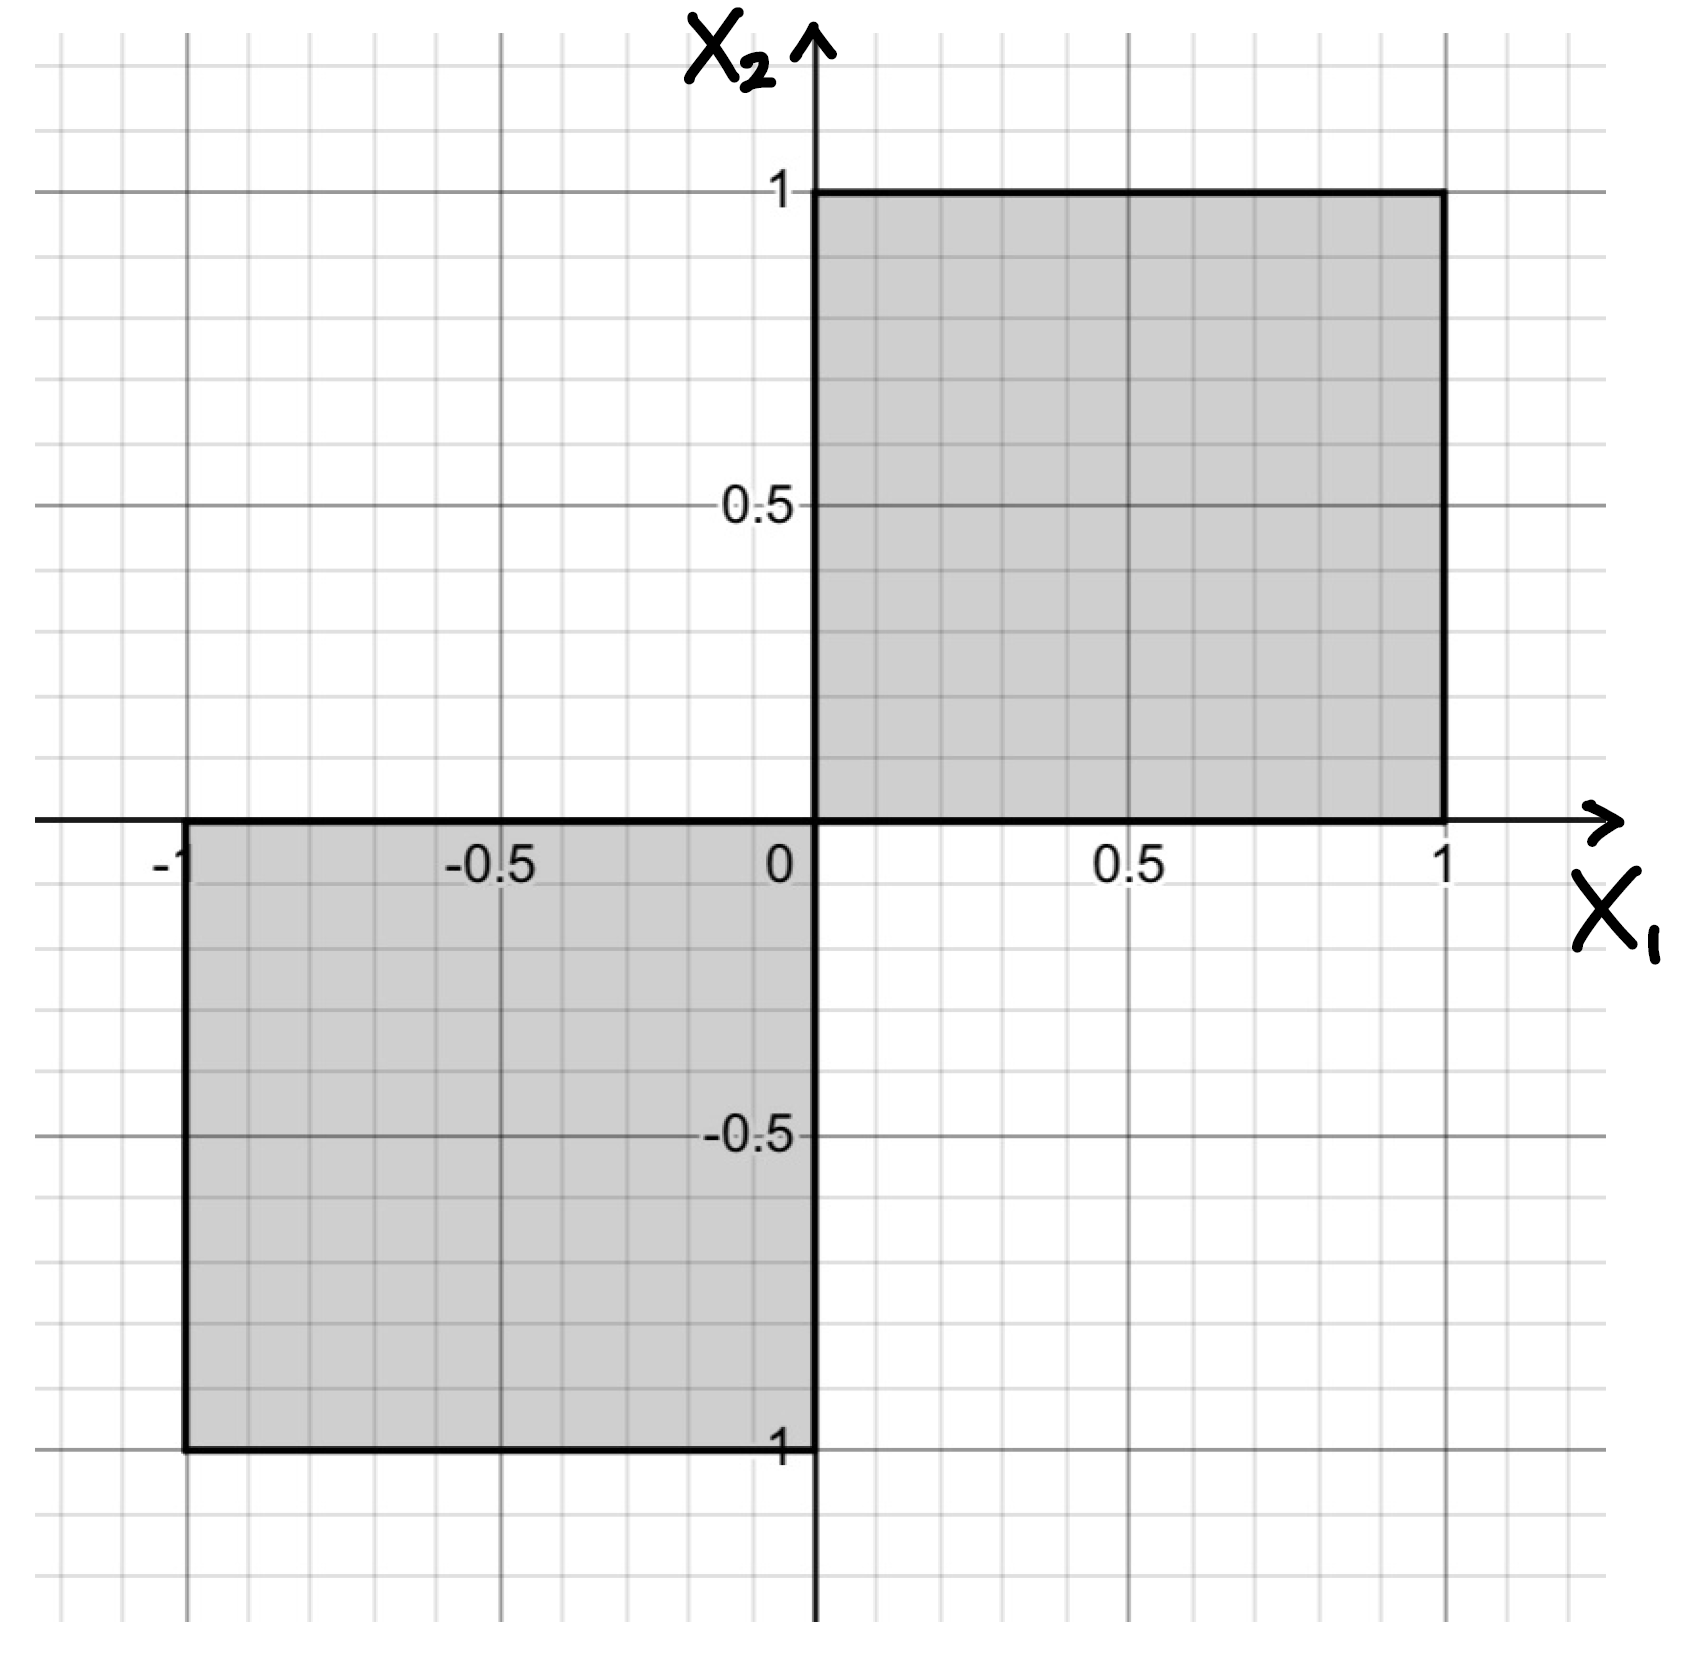
\includegraphics[width=.35\textwidth]{images/scribe19_image3.png}
  \caption{Distribution of \((X_1,X_2)\).}
  \label{fig3}
\end{figure}

Allocate \(R=2\) bits per component and apply the scalar quantizer
\[
Q(x)=
\begin{cases}
0\,(00), & x\in[-1,-0.5),\\
1\,(01), & x\in[-0.5,0),\\
2\,(10), & x\in[0,0.5),\\
3\,(11), & x\in[0.5,1].
\end{cases}
\]
Figure~\ref{fig4a} shows the resulting \(4 \times 4\) grid in the 
\((X_1,X_2)\)-plane.  
Because some codewords correspond to impossible source outcomes (white squares), 
bits are wasted.  
A finer VQ with 16 properly shaped regions (Figure~\ref{fig4b}) eliminates this waste 
and yields lower mean-squared distortion.

\begin{figure}[ht]
  \centering
  \begin{subfigure}{0.4\textwidth}
    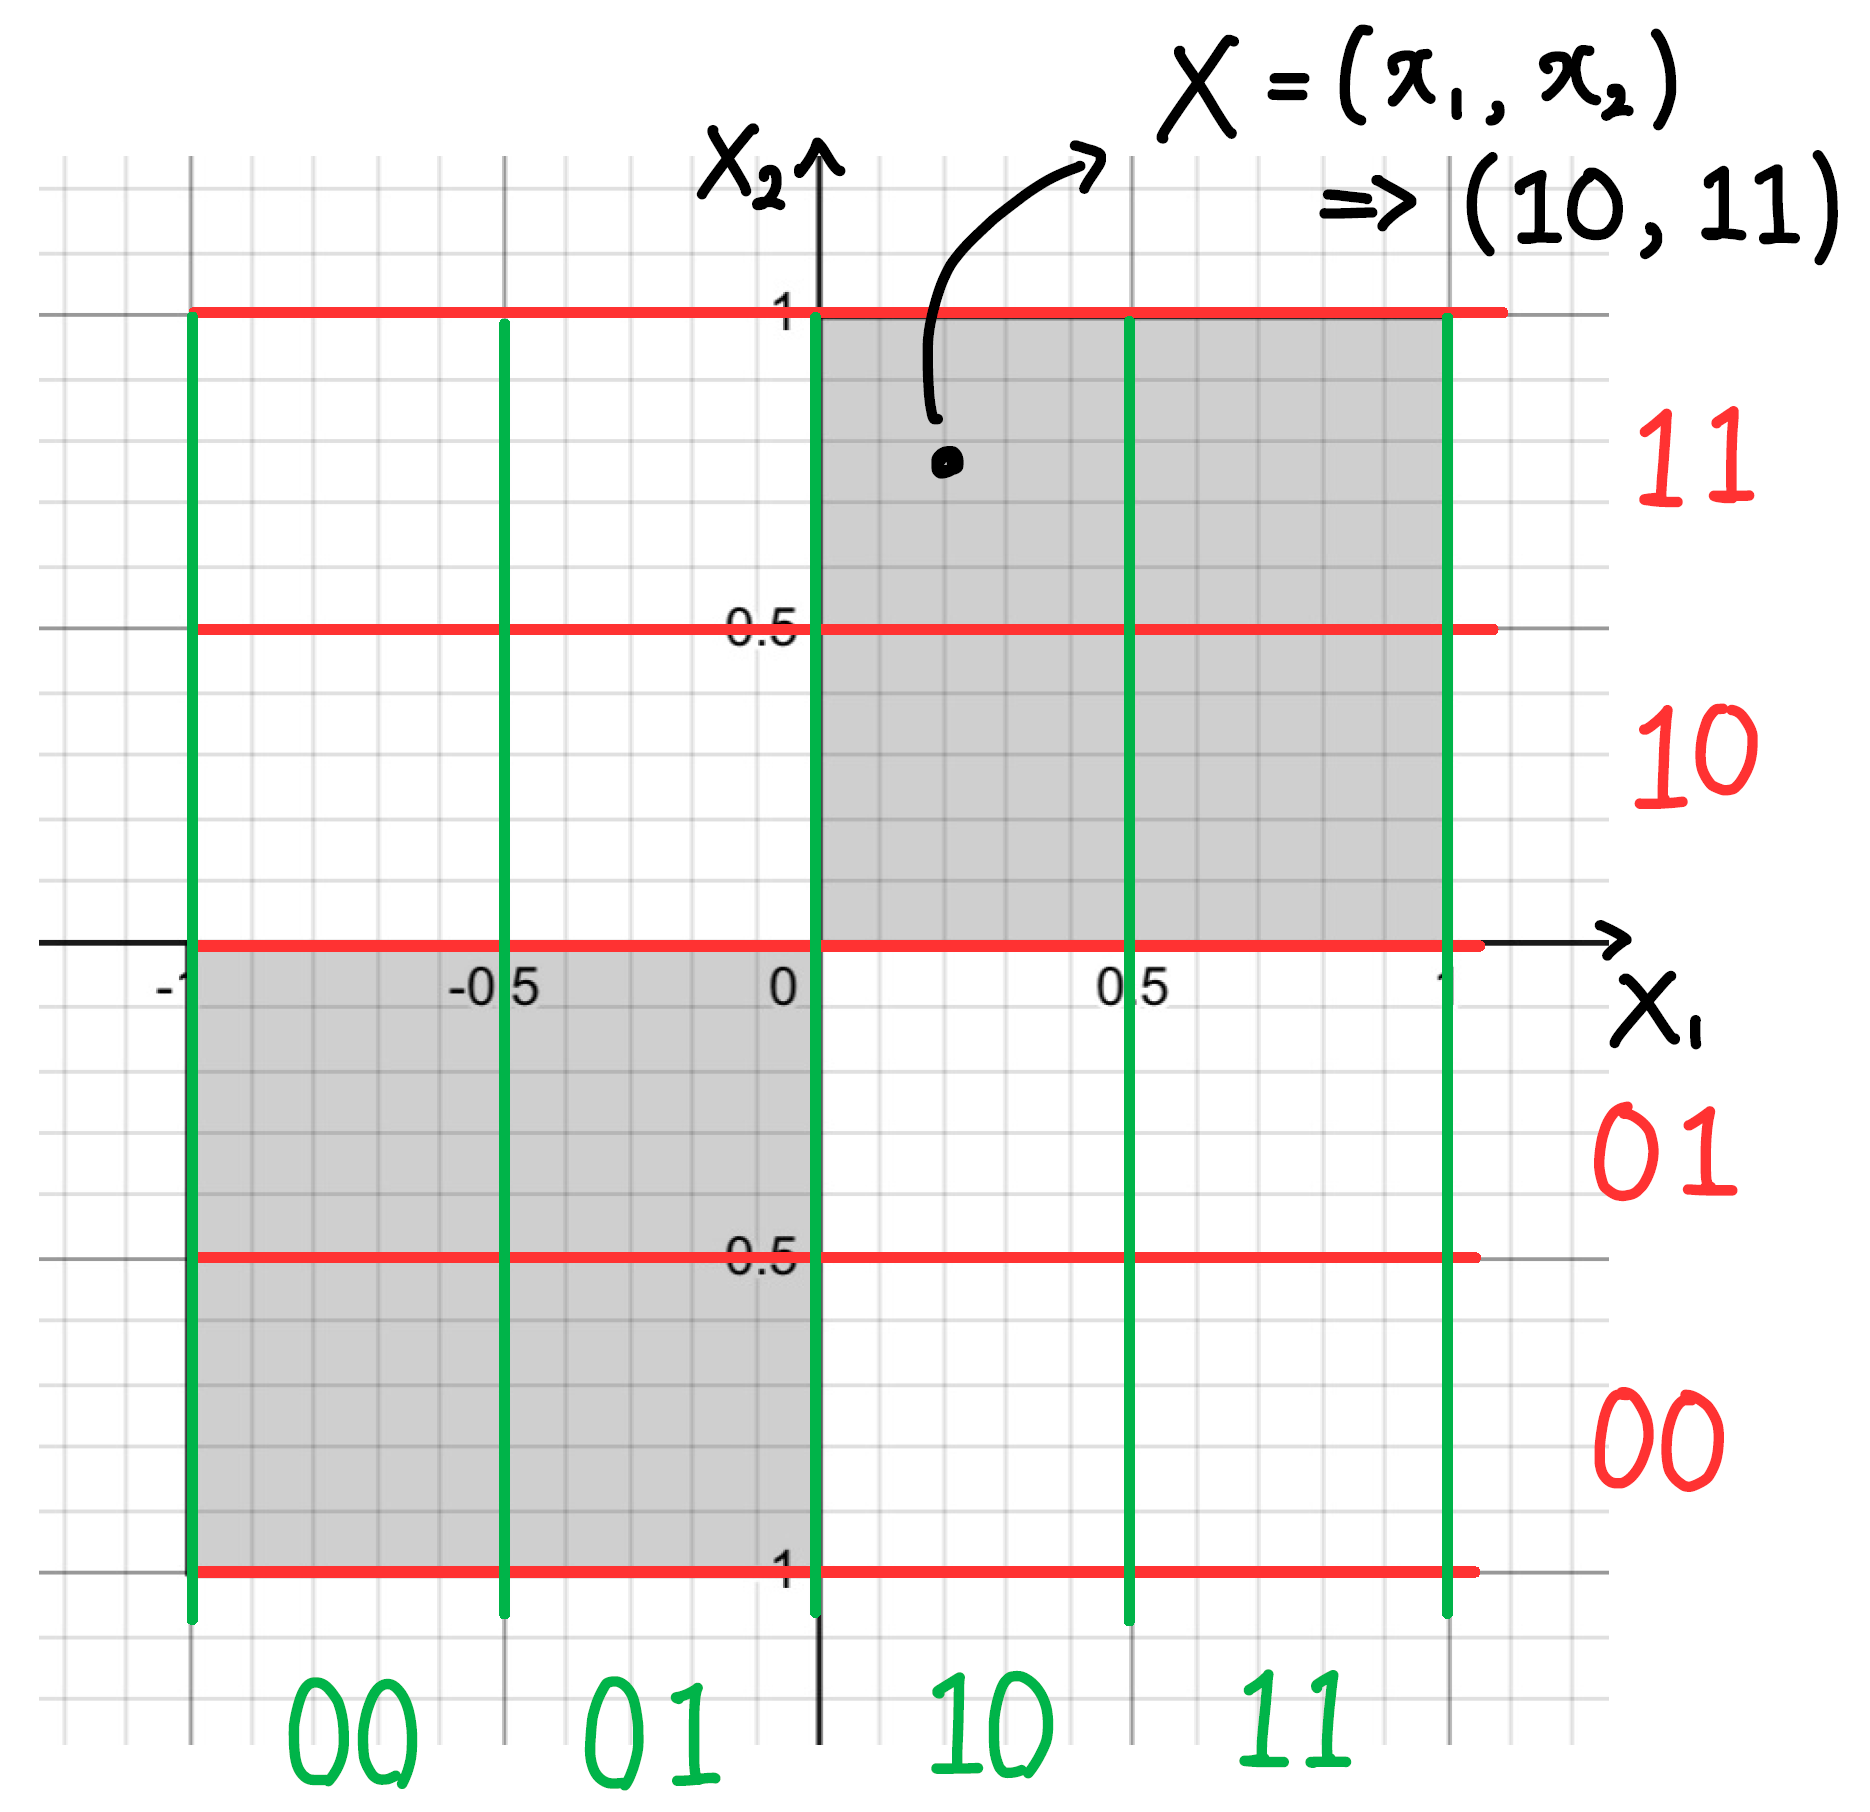
\includegraphics[width=\linewidth]{images/scribe19_image4a.png}
    \caption{Scalar quantization.}
    \label{fig4a}
  \end{subfigure}\hspace{10mm}
  \begin{subfigure}{0.37\textwidth}
    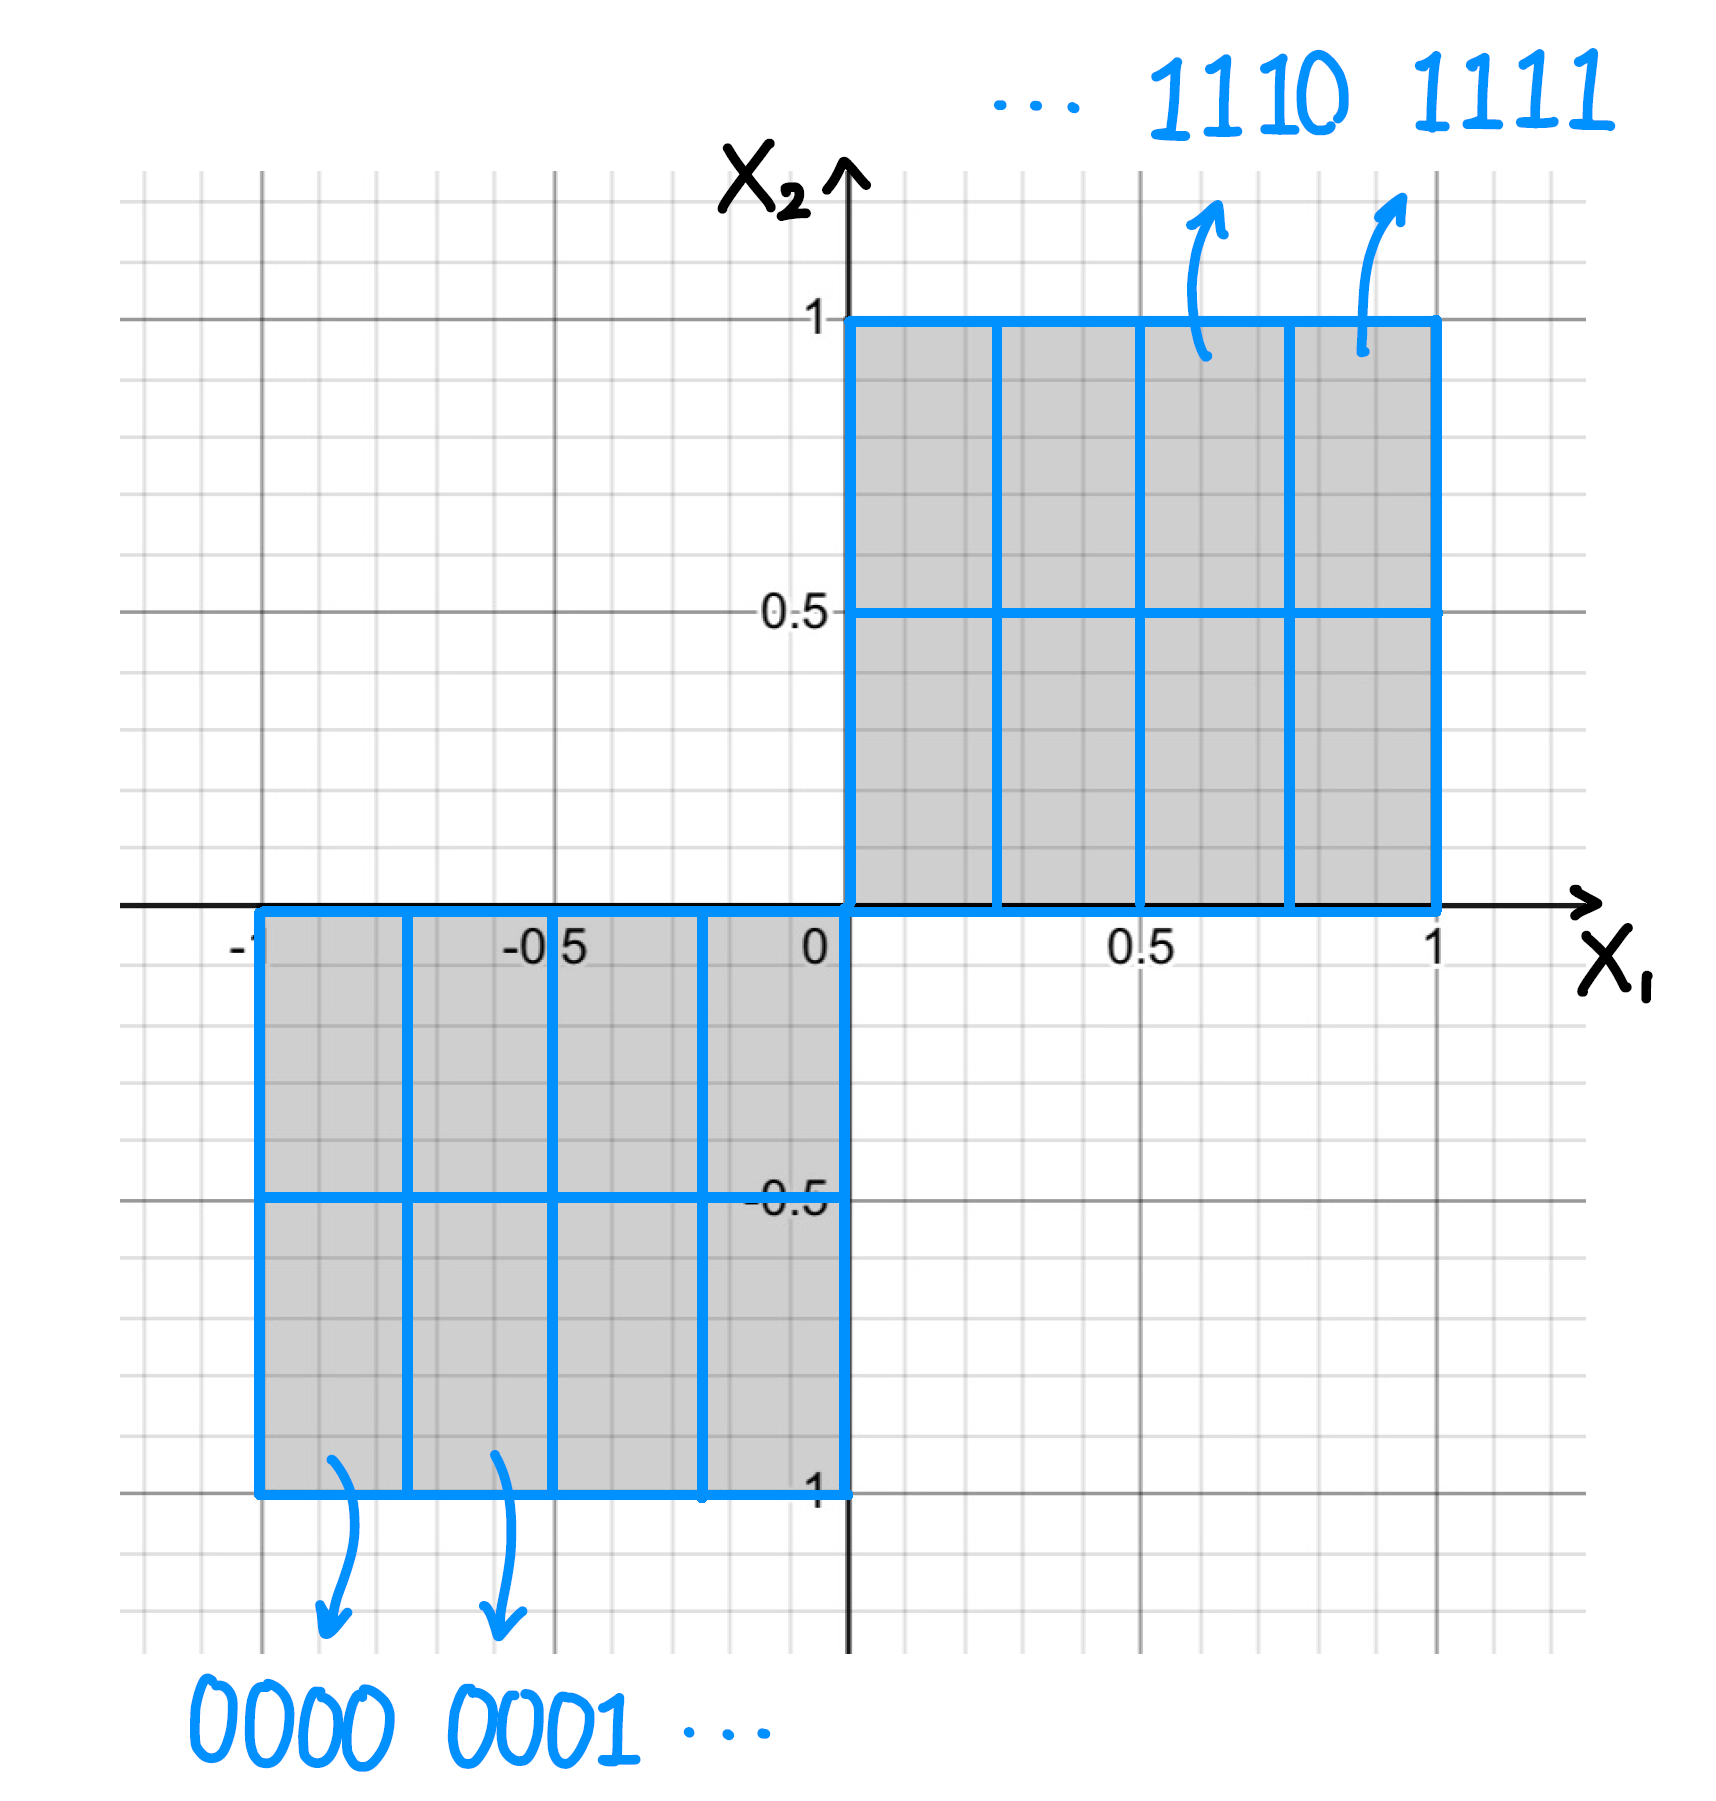
\includegraphics[width=\linewidth]{images/scribe19_image4b.png}
    \caption{Vector quantization (16 clusters).}
    \label{fig4b}
  \end{subfigure}
  \caption{Scalar vs.\ vector quantization.}
  \label{fig4}
\end{figure}
\end{example}

In general, the reconstruction error is minimized when each region is 
close to circular; rectangular cells created by scalar quantization are 
non-elastic and therefore sub-optimal (Figure~\ref{fig:distortion}).

\begin{figure}[ht]
  \centering
  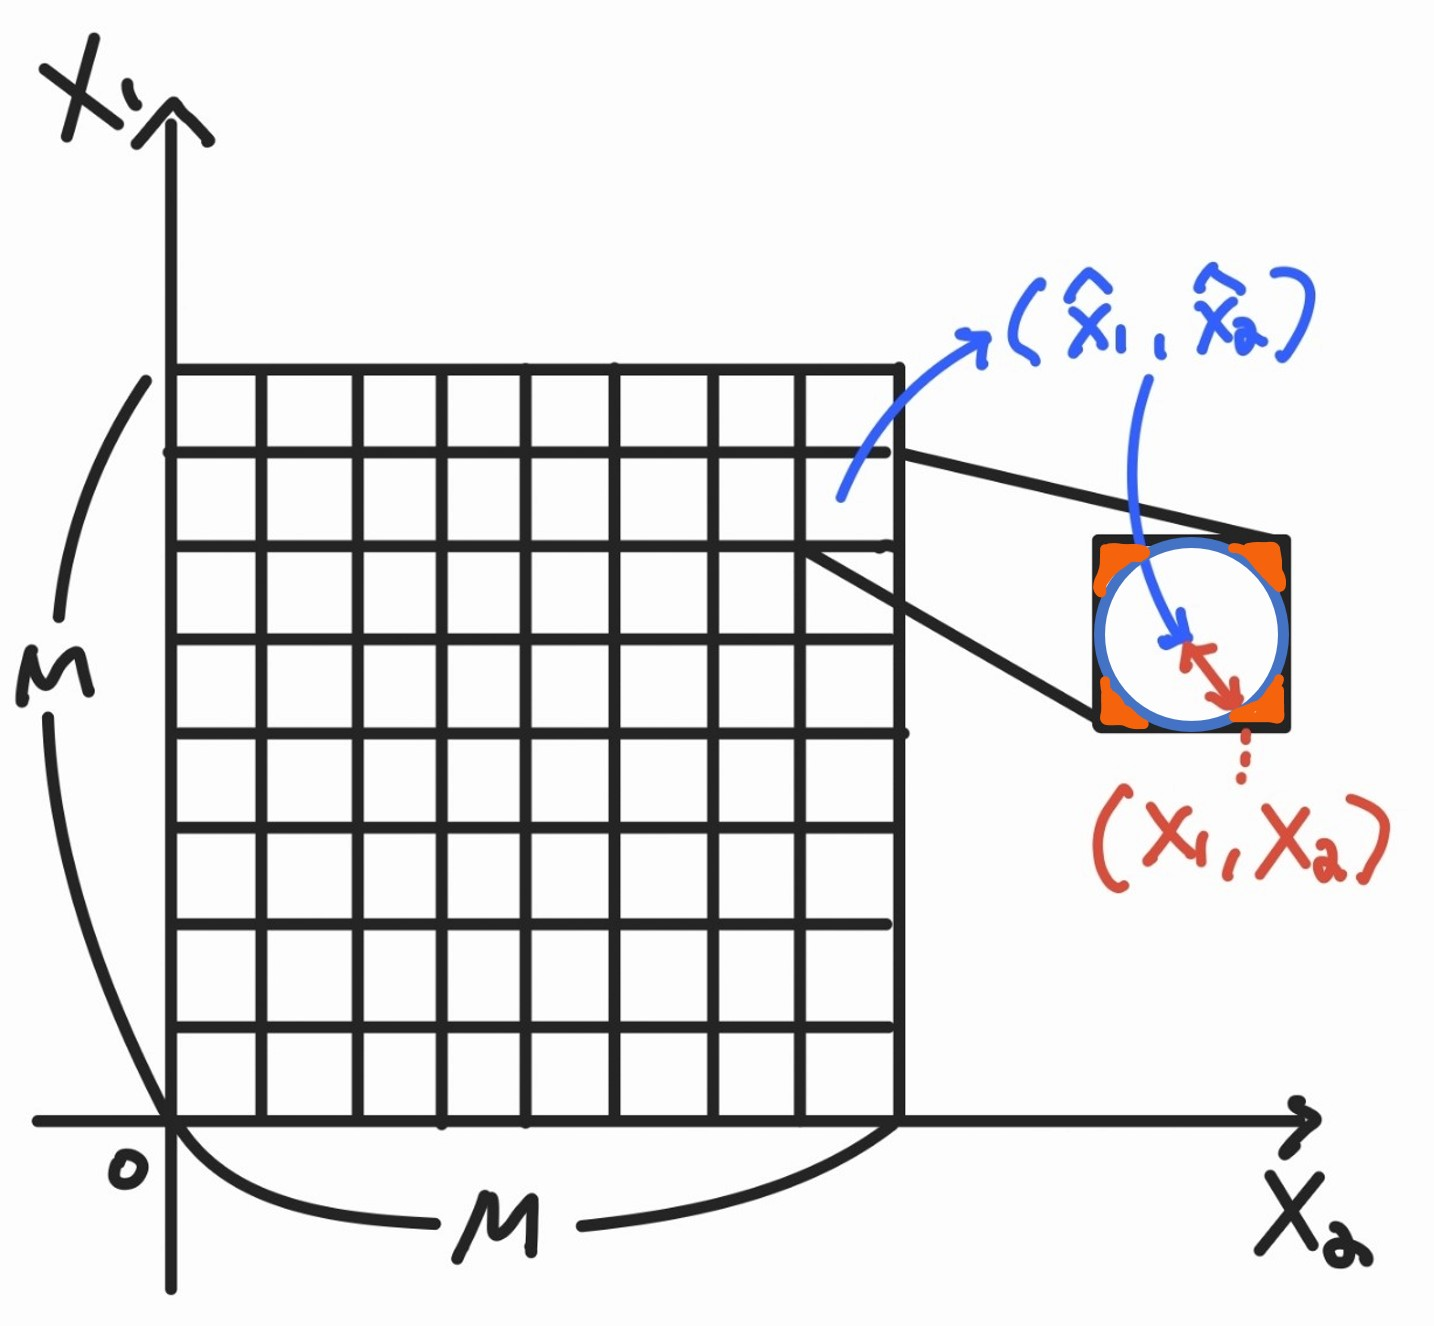
\includegraphics[width=0.3\textwidth]{images/scribe19_Figure3.jpg}
  \caption{Additional distortion caused by rigid, rectangular cells.}
  \label{fig:distortion}
\end{figure}

\subsubsection*{Vector quantization strictly improves distortion}

Even when the source components are independent, VQ achieves a strictly 
lower rate–distortion trade-off than scalar quantization because it can 
jointly shape the cells.

\begin{example}
For the same 2-D uniform source, Figure~\ref{fig5} compares the optimal 
representatives of (a) a scalar \(M\times M\) grid and (b) a VQ with 
hexagonal (approximately circular) cells.  
The red arrows indicate quantization errors; the hexagonal tessellation 
yields uniformly shorter arrows and hence smaller distortion.

\begin{figure}[ht]
  \centering
  \begin{subfigure}{0.5\textwidth}
    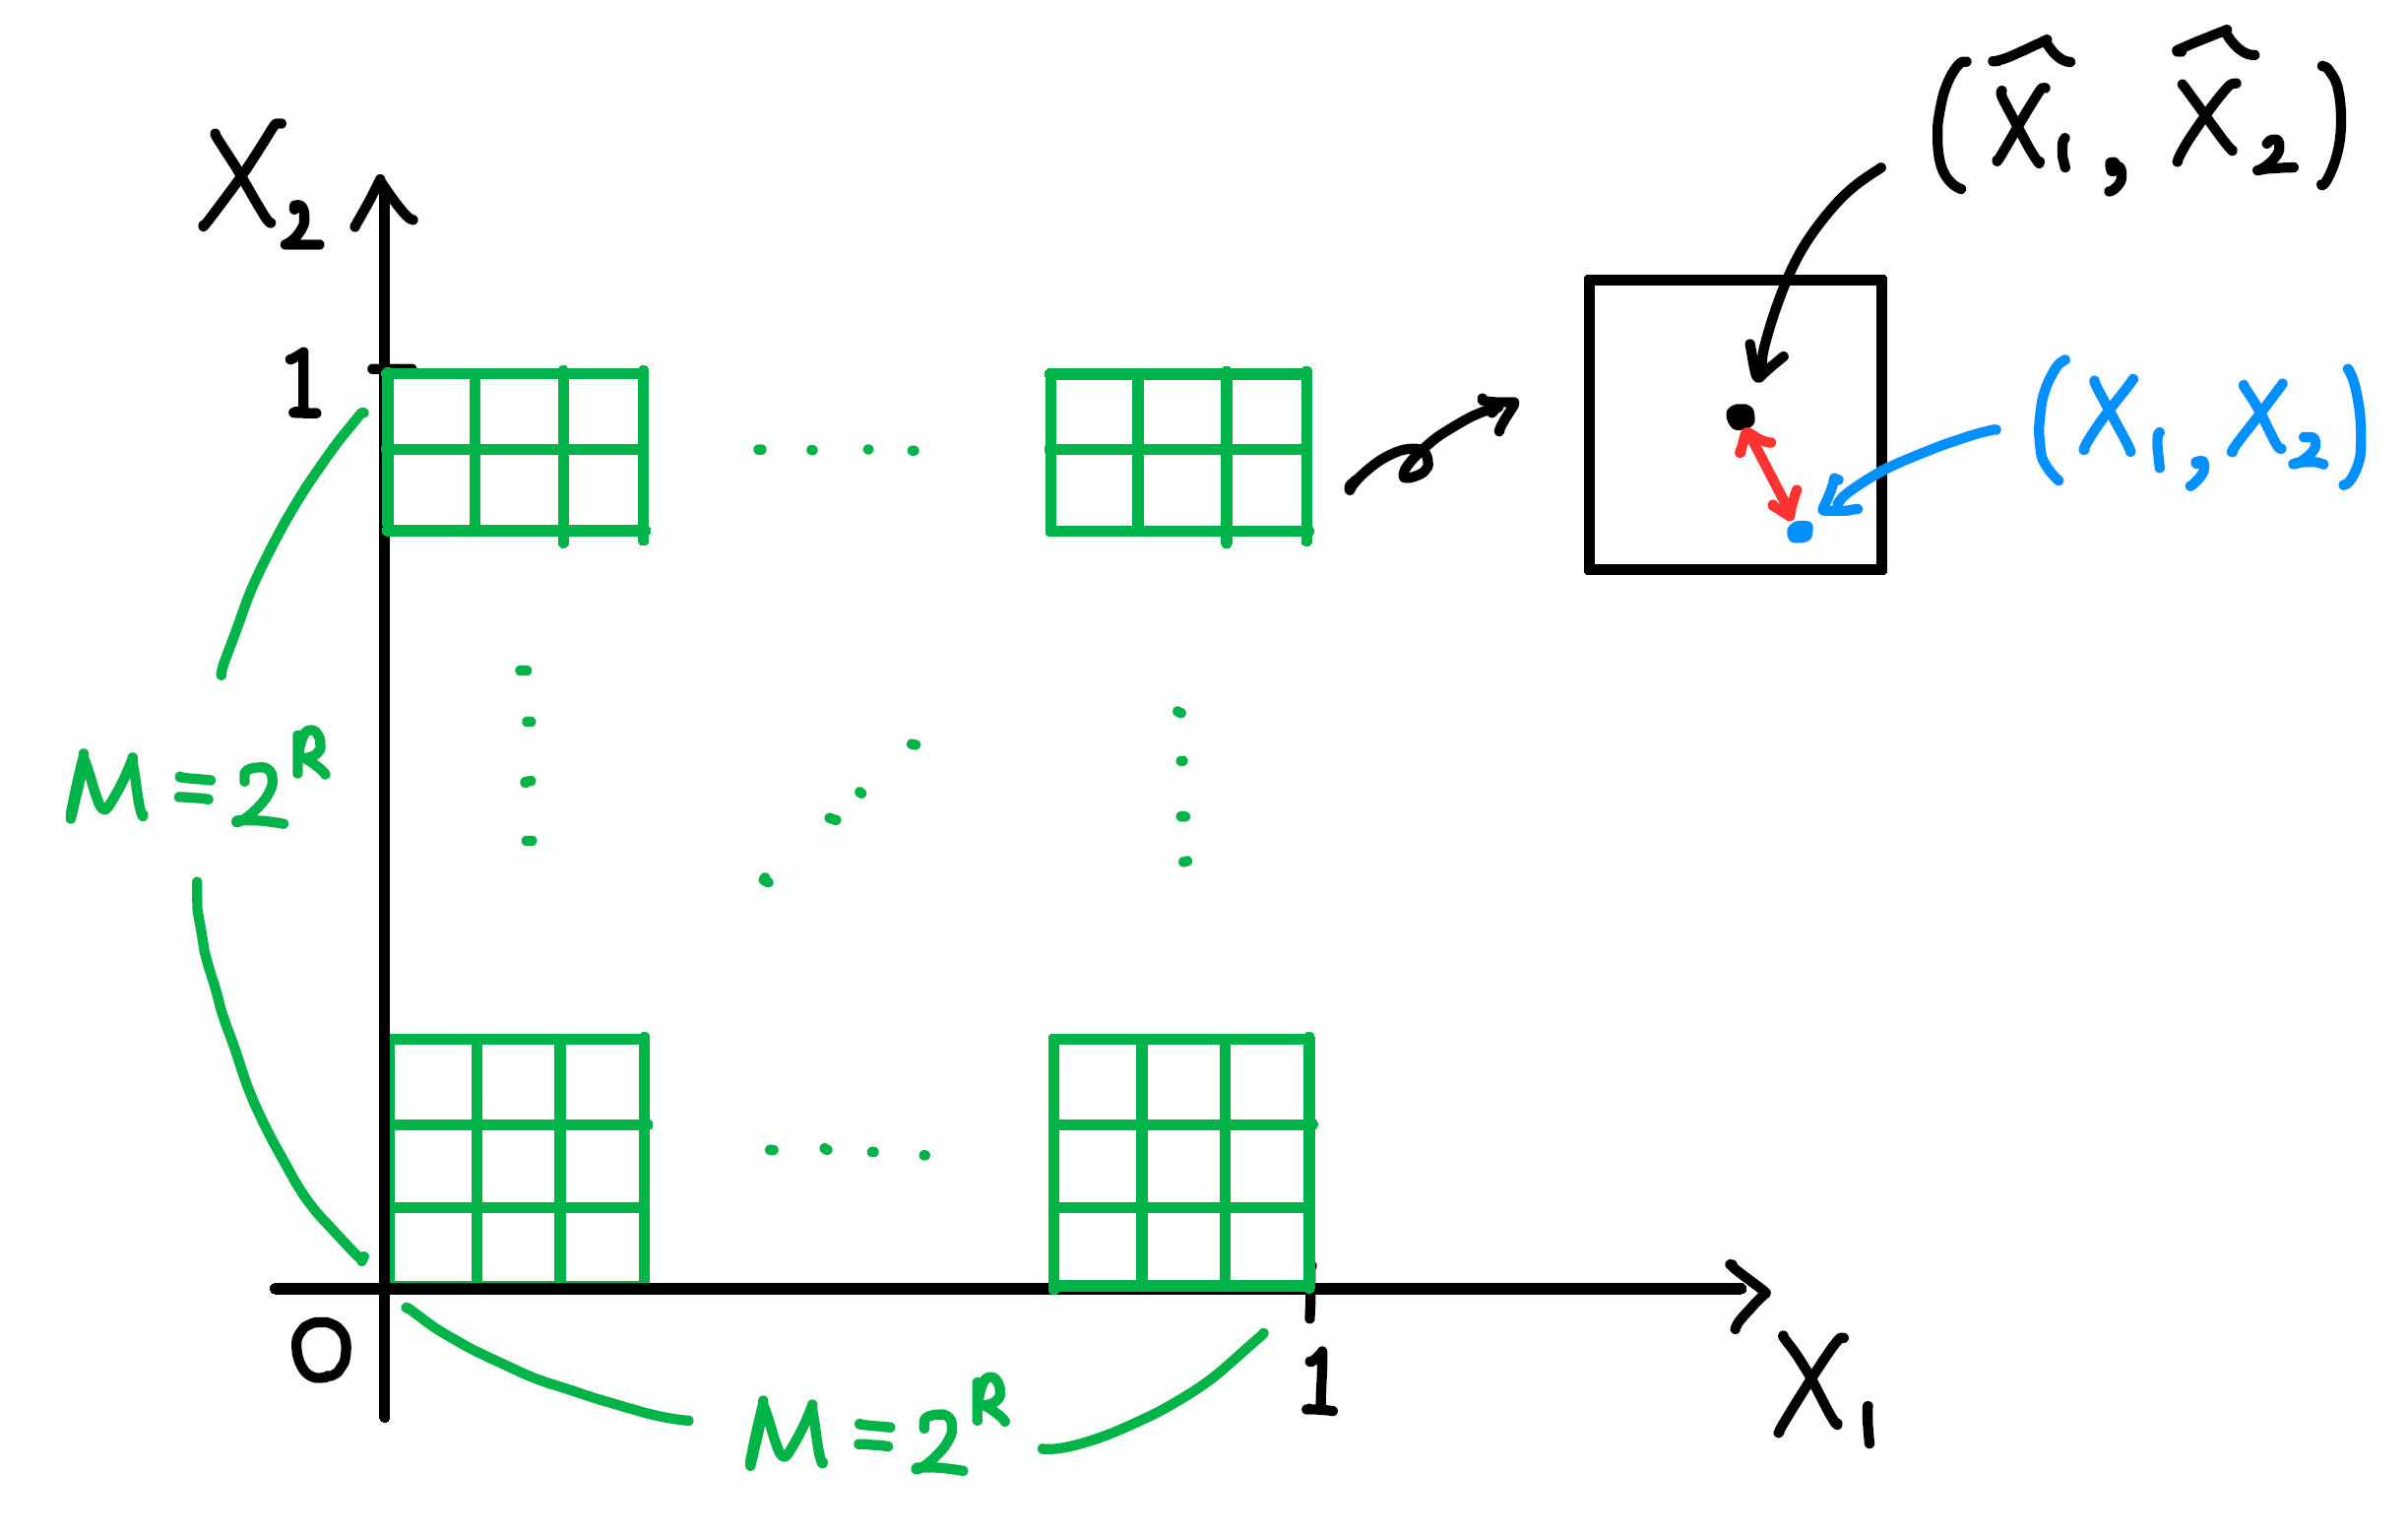
\includegraphics[width=\linewidth]{images/scribe19_image5a.png}
    \caption{Scalar \(M\times M\) grid.}
    \label{fig5a}
  \end{subfigure}\hspace{1mm}
  \begin{subfigure}{0.43\textwidth}
    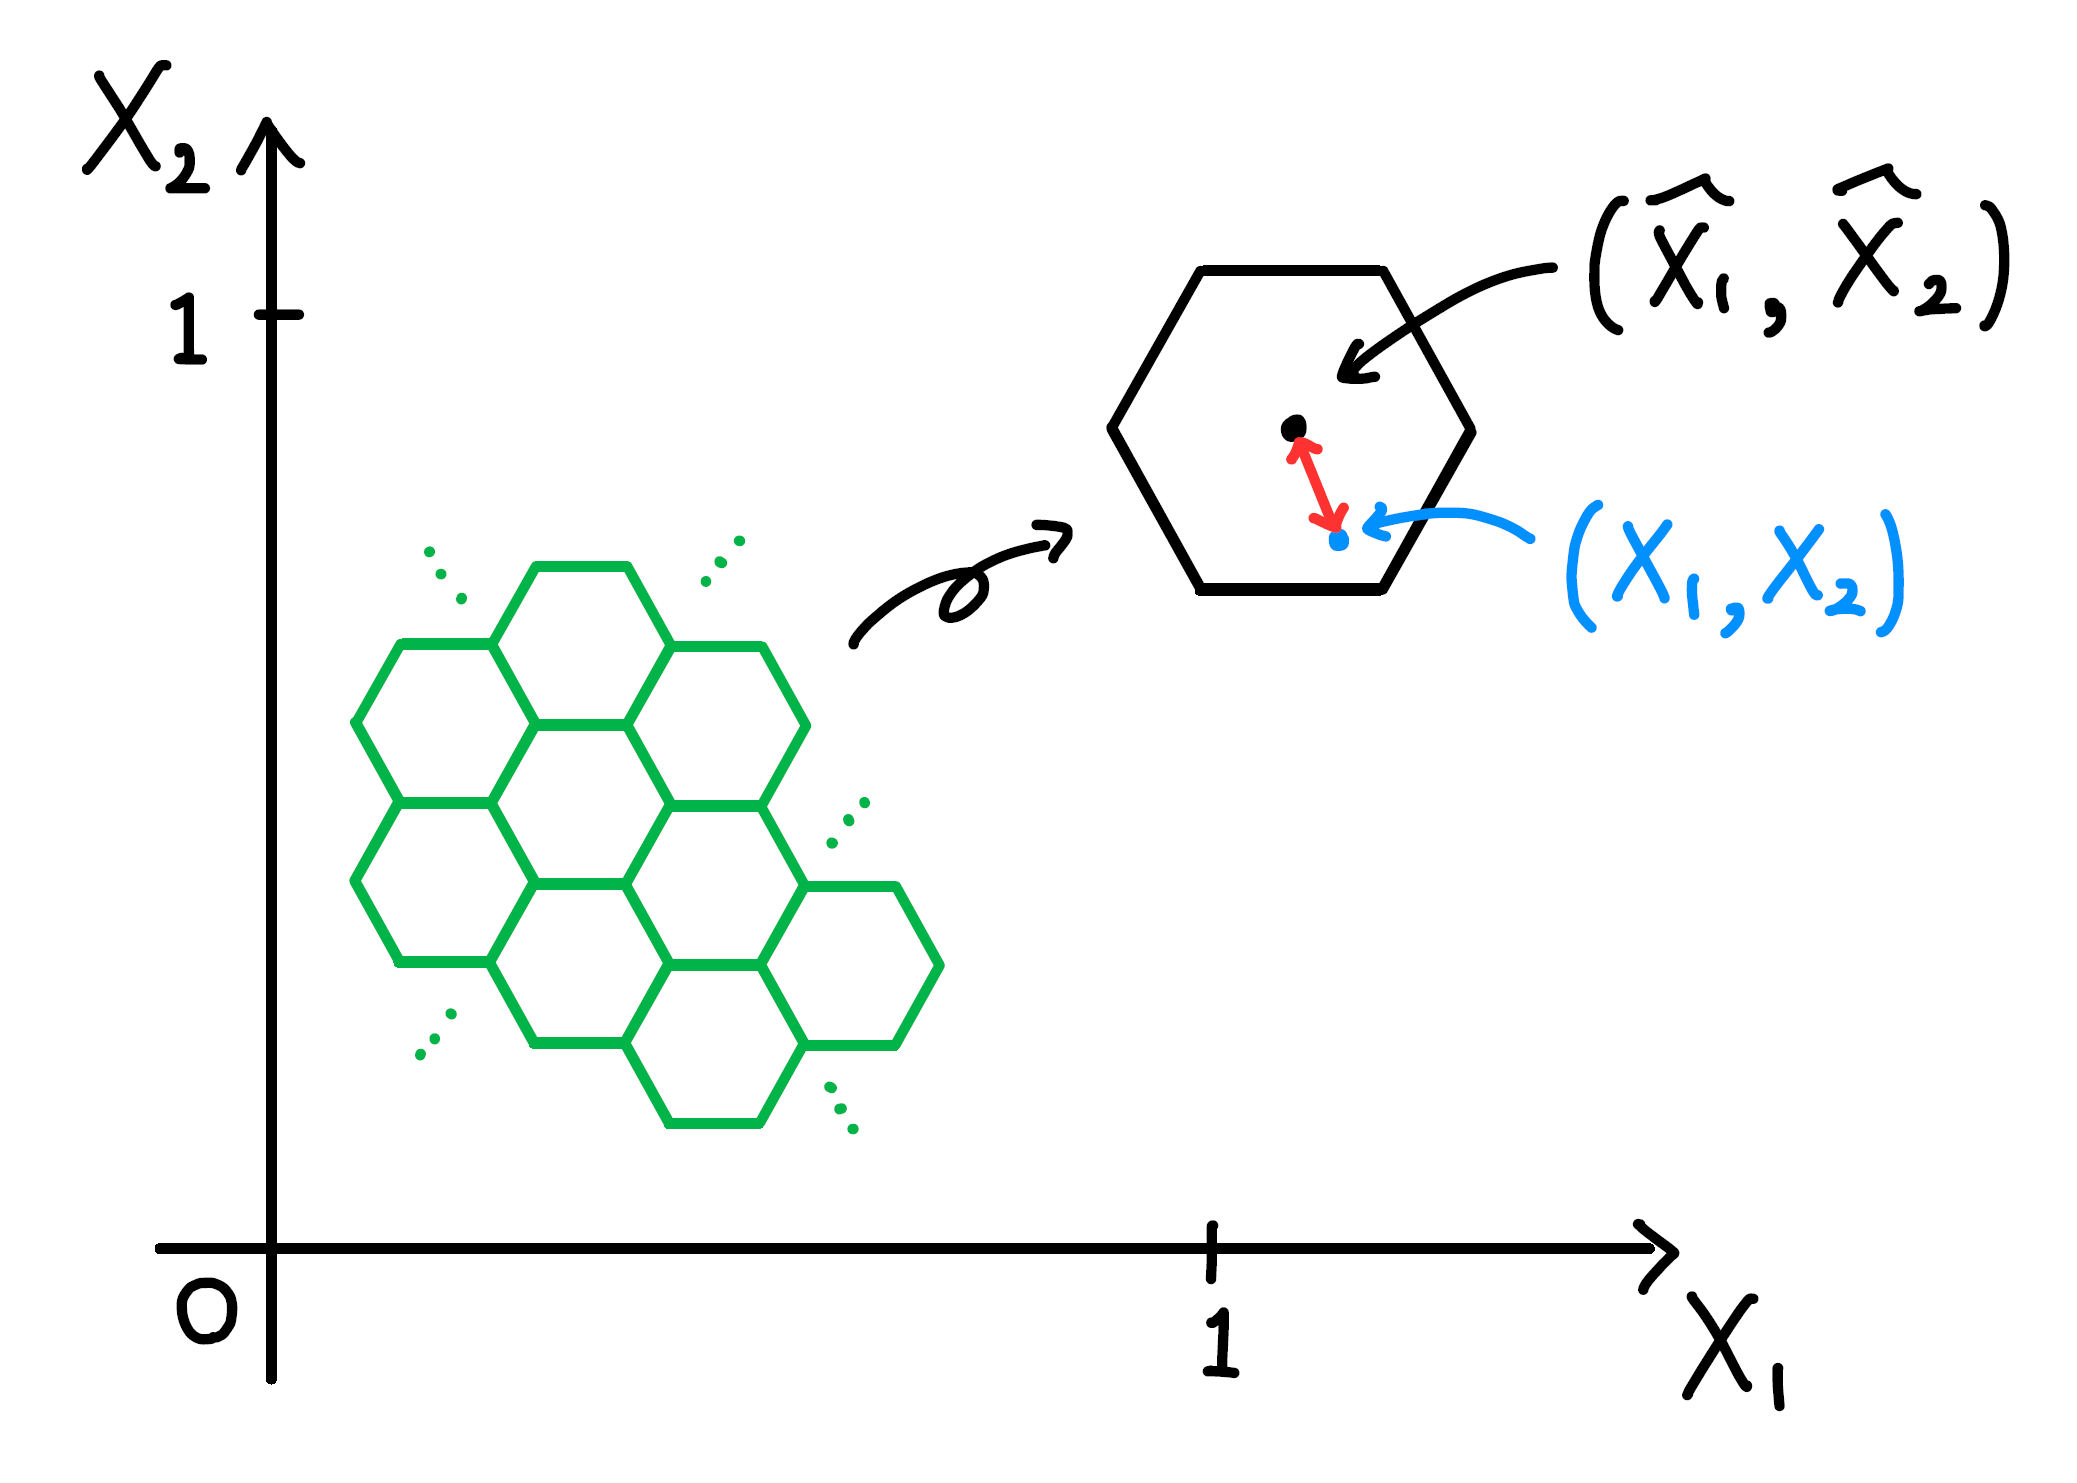
\includegraphics[width=\linewidth]{images/scribe19_image5b.png}
    \caption{Vector quantization with hexagonal cells.}
    \label{fig5b}
  \end{subfigure}
  \caption{Distortion comparison: rectangular vs.\ circle-like cells.}
  \label{fig5}
\end{figure}
\end{example}
%%%%%%%%%%%%%%%%%%%%%%%%%%%%%%%%%%%%%%%%%%%%%%%%%%%%%%%%%%%%%%%%%%%%%%%%
\subsection{Rate–Distortion Theory}
\label{sec:RD}
\subsubsection*{Recap}
A vector quantizer of block-length \(n\) is a pair
\[
f:\mathcal X^{n}\!\longrightarrow\{0,\dots,M\!-\!1\},\qquad
g:\{0,\dots,M\!-\!1\}\!\longrightarrow\widehat{\mathcal X}^{n},
\]
with \(M=2^{nR}\).  
The encoder transmits the index \(m=f(X^{n})\) at an average rate
\(R\) bits/symbol and the decoder outputs
\(\widehat X^{n}=g(m)\).
Given a single-letter distortion measure \(d:\mathcal X\times\widehat{\mathcal X}\!\to\!\mathbb R_{\ge0}\),
the block distortion is the sample mean
\(d^{(n)}(x^{n},\widehat x^{n})=\frac1n\sum_{i=1}^{n}d(x_i,\widehat x_i)\).

\subsubsection*{Information-theoretic form}

Let \(X\sim P_X\) be i.i.d.\ and let
\(d:\mathcal X\times\widehat{\mathcal X}\to\mathbb R_{\ge0}\).

\begin{definition}
\((R,D)\) is \emph{achievable} if for every \(\varepsilon>0\) and all
sufficiently large \(n\) there exists an \((n,R+\varepsilon)\) code
with
\(\displaystyle
\mathbb E[d^{(n)}(X^{n},\widehat X^{n})]\le D+\varepsilon\).
\end{definition}

\begin{definition}[Information Rate-Distortion Function]
    The information rate-distortion function $R^{(I)}(D)$ is defined as
    \[
    R^{(I)}(D) = \inf_{\mathbb{E}[d(X, \widehat{X})] \leq D} I(X; \widehat{X}).
    \]
\end{definition}

\begin{theorem}[Shannon's Rate-Distortion Theorem]\label{thm:shannonRD}
\(R(D)=R^{(I)}(D)\) for every memoryless source and single-letter
distortion.
\end{theorem}

\begin{definition}[Jointly Typical set]
    For $n$-length random sequences $x^n$ and $y^n$, the jointly typical set is defined as
    \[
A_\varepsilon^n := 
\left\{
\begin{aligned}
(x^n, y^n):\quad
& p(x^n)       \approx 2^{-nH(X)} \\
& p(y^n)       \approx 2^{-nH(Y)} \\
& p(x^n, y^n)  \approx 2^{-nH(X,Y)}
\end{aligned}
\right\}.
\]
\end{definition}

\begin{lemma}
The probability that a tuple of independent sequences $(X^n,Y^n)$ belongs to a jointly typical set is approximately $2^{-nI(X;\,Y)}$.

\begin{proof}
    $|A_{\epsilon}^n|$ is approximately $2^{nH(X,Y)}$. (Why?)
    Then \[\begin{aligned}\text{Pr}\{(X^n,Y^n)\in A_\epsilon^n\}&=\sum _{(x^n,
    \,y^n)\in A_{\epsilon}^n}p(x^n,\,y^n)\\&=\sum _{(x^n,
    \,y^n)\in A_{\epsilon}^n}p(x^n)p(y^n)\\&\approx|A_{\epsilon}^n|\cdot2^{-nH(X)}\cdot2^{-nH(Y)}\\&=2^{n(H(X,Y)-H(X)-H(Y))}=2^{-nI(X;Y)}.\end{aligned}\]
\end{proof}
\end{lemma}

\begin{example}[Binary source with Hamming distortion]

For \(X\sim\mathrm{Bern}(p)\,(p\leq \frac12)\) and
\(d_H(x,\widehat x)=\mathbf1\{x\ne\widehat x\}\), 
\[
R(D)=\begin{cases}
H_2(p)-H_2(D), & 0\le D\le p,\\[2pt]
0,             & D\ge p.
\end{cases}
\]

\begin{proof}
If $D\geq p$, we don't need any description. Consider 
\[\begin{aligned}I(X;\widehat{X}) &= H(X)-H(X\,|\,\widehat{X})\\&=H_2(p)-H(X\oplus\widehat{X}\,|\,\widehat{X})\\&=H_2(p)-H(X\oplus\widehat{X})\\&=H_2(p)-H_2(\text{Pr}(X\neq \widehat{X}))\\&\geq H_2(p)-H_2(D).\end{aligned}\]
We need to show this lower bound can be achieved; Let $\widehat{X} \sim \mathrm{Bern}(q)$ and $Z\sim \mathrm{Bern}(D)$, which is independent of $\widehat{X}$. Setting $X=\widehat{X}\oplus Z$ gives $q=\frac{p-D}{1-2D}$ (so that $\text{Pr}(X=1)=p$).\\
\textbf{Generation of codebook.} Generate $M=2^{nR}$ reconstruction sequences $\widehat{x}(0),\,\widehat{x}(1),\,...,\,\widehat{x}(M-1) \overset{\text{i.i.d}}{\sim} \mathrm{Bern}(q)$. Given a source block $x^n,$ scan the codebook; find an index $m$ such that the pair $(x^n,\widehat{x}^n(m))$ is jointly typical with respect to the $P_{X,\widehat{X}}$. Jointly typical means that their empirical joint frequencies are within $\epsilon$ of the true probabilities. If at least one such $m$ exists, transmit it. Otherwise, declare an encoding error. Whenever a jointly typical pair is found, the empirical error rate of the block satisfies 
$$
\left|\frac{1}{n}\sum_{i=1}^n\mathbf{1}_{\{x_i\neq\widehat{x}_i\}}-D\right|\leq\epsilon,
$$
Hence the expected block distortion $\mathbb{E}[d_H(X,\widehat{X})]\approx D$ as $n\to\infty$ by the Law of Large Number. Given a source sequence $x^n$, for a random codeword $\widehat{x}^n,$ the probability that $(x^n,\,\widehat{x}^n)$ is jointly typical is roughly $2^{-nI(X;\,\widehat{X})}$. The $2^{nR}$ codewords are independent, so

$$P_\text{error}\leq(1-2^{-nI(X;\,\widehat{X})})\approx \exp(-2^{n(R-I)})\overset{n\to\infty}{\longrightarrow}0\quad\text{if}\,\,R>I(X;\widehat{X}).$$

\end{proof}
\end{example}

\begin{example}[Gaussian source with quadratic distortion]

For a zero–mean Gaussian source \(X\sim\mathcal N(0,\sigma^{2})\) and
squared-error distortion \(d_2(x,\widehat x)=(x-\widehat x)^{2}\),
\[
R(D)=
\begin{cases}
\displaystyle\frac12\log_{2}\!\Bigl(\frac{\sigma^{2}}{D}\Bigr),
        & 0<D\le\sigma^{2},\\[6pt]
0,      & D\ge\sigma^{2}.
\end{cases}
\]

\begin{proof}
\(R^{(I)}(D)=\underset{P_{X,\widehat X}:\,\mathbb{E}[(X-\widehat X)^2]\leq D}{\underset{P_X\sim\mathcal{N}(0,\sigma^2)}{\inf}}I(X;\widehat X)\). We get lower bound as follows:
\[
\begin{aligned}
    I(X;\widehat X)&=h(X)-h(X\,|\,\widehat X)\\
    &=\frac12\log2\pi e\sigma^2-h(X-\widehat X\,|\,\widehat X)\\&\geq\frac12\log2\pi e\sigma^2-h(X-\widehat{X})\\&\geq\frac12\log2\pi e\sigma^2-\frac12\log2\pi eD\\&=\frac12\log\frac{\sigma^2}{D}.
\end{aligned}
\]
We need to prove achievability. choose an independent test channel \(Z\sim\mathcal N(0,D)\) and set
\(X=\widehat X+Z\). Then \(\widehat X\) is Gaussian with variance \(\sigma^{2}-D\) and \(\mathbb E[(X-\widehat X)^{2}]=D\).\\  

\noindent\textbf{Generation of codebook.}
Generate $M=2^{nR}$ reconstruction sequences $\widehat{x}(0),\,\widehat{x}(1),\,...,\,\widehat{x}(M-1) \overset{\text{i.i.d}}{\sim}\mathcal{N}(0,\sigma^2-D)$. Given a source block $x^n$, find a jointly typical $\widehat x^n(m)$. The probability that we get a jointly typical $\widehat x^n$ is roughly $2^{-nI(X;\widehat X)}.$ So, if $R>I(X;\widehat X),$ we can encode $x^n$ without an error with high probability as $n\to\infty$, same as before.
\end{proof}
\end{example}

\paragraph{Intuitive explanation}\label{subsec:intuition}

For a large block length \(n\) we can view each realization
\(
X^{n}=(X_{1},\dots,X_{n})
\)
as a point in \(\mathbb R^{n}\).
By the law of large numbers
\[
\frac1n\|X^{n}\|^{2}
    =\frac1n\sum_{i=1}^{n}X_{i}^{2}
    \;\xrightarrow{\;n\to\infty\;}\;
    \mathbb E[X^{2}]
    =\sigma^{2},
\qquad
\text{i.e.}\quad
\|X^{n}\|\approx\sqrt{n\sigma^{2}}.
\]
Hence, with overwhelming probability the source vectors lie near the
surface of an \(n\)-sphere of radius \(\sqrt{n\sigma^{2}}\).

For the test channel used in the achievability proof we write
\(X=\widehat X+Z\) with \(Z\sim\mathcal N(0,D)\) independent of
\(\widehat X\).
Then \(\operatorname{Var}(\widehat X)=\sigma^{2}-D\), so
\[
\|\widehat X^{n}\|\approx\sqrt{n(\sigma^{2}-D)}.
\]
Geometrically, the \(2^{nR}\) reconstruction points
\(\widehat X^{n}(m)\)
concentrate on a slightly smaller sphere.

\paragraph{Covering argument (converse).}
Fix a reproduction block \(\widehat x^{n}\).
To keep the block distortion below \(D\) we must map every
source vector inside the radius-\(\sqrt{nD}\) ball centred at
\(\widehat x^{n}\), because
\[
\|X^{n}-\widehat X^{n}\|^{2}
      =\sum_{i=1}^{n}(X_{i}-\widehat X_{i})^{2}
      \approx n\mathbb E[(X-\widehat X)^{2}]
      \le nD.
\]
Let \(V_{n}\) be the volume of the unit \(n\)-ball.
Then

\[
\underbrace{V_{n}\bigl(\sqrt{n\sigma^{2}}\bigr)^{n}}
_{\text{volume of the source shell}}
\;\le\;
2^{\,nR}\;
\underbrace{V_{n}\bigl(\sqrt{nD}\bigr)^{n}}
_{\text{volume covered by one codeword}},
\]
otherwise some source points could not be matched within distortion
\(D\).
Cancelling \(V_{n}\) and taking \(\log\) gives the fundamental lower
bound
\[
R\;\ge\;\frac12\log\frac{\sigma^{2}}{D}.
\]

Because the achievability part already built a code that meets this
rate, the geometric covering argument certifies that the bound is
tight; no smaller rate can satisfy the distortion constraint.  Thus the
operational rate–distortion function equals
\(R(D)=R^{(I)}(D)=\tfrac12\log_{2}(\sigma^{2}/D)\).

\medskip
\begin{example}[Laplacian source with absolute distortion]

Let the source be
\(X\sim\mathrm{Lap}(1/\lambda)\) with pdf
\(f_X(x)=\tfrac{\lambda}{2}e^{-\lambda|x|}\)
and let the distortion measure be
\(d_1(x,\widehat x)=|x-\widehat x|\).
Then
\[
R(D)=
\begin{cases}
       -\log(\lambda D),
         & 0<D\le\frac1{\lambda},\\[6pt]
0,      & D\ge\frac1{\lambda}.
\end{cases}
\]

\begin{proof}
Define the auxiliary conditional
\(Q_{X|\widehat X}(x|\widehat x)
      =\frac1{2D}\exp\!\bigl(-|x-\widehat x|/D\bigr),
      \quad\text{i.e.\ }X|\widehat X\sim\mathrm{Lap}(\widehat x,D).\) For any feasible joint law \(P_{X,\widehat X}\) with
\(\mathbb E|X-\widehat X|\le D\),

\[
\begin{aligned}
    I(X;\widehat X)&=\mathbb{E}\left[\log\frac{p(X\,|\,\widehat X)}{p(X)}\right]\\&=\mathbb{E}\left[\log\frac{p(X\,|\,\widehat X)}{q(X\,|\,\widehat X)}\right]+\mathbb{E}\left[\log\frac{q(X\,|\,\widehat X)}{p(X)}\right]\\&=D_{KL}(P_{X|\widehat X}\,||\,Q_{X|\widehat X})+\mathbb{E}\left[\log\frac{q(X\,|\,\widehat X)}{p(X)}\right]\\&\geq\mathbb{E}\left[\log\frac{q(X\,|\,\widehat X)}{p(X)}\right].
\end{aligned}
\]
Choosing \(P_{X|\widehat X}=Q_{X|\widehat X}\) makes the KL term zero, so
\[
I(X;\widehat X)\;\ge\;
h(X)-h_Q(X|\widehat X)
      =\log(2e/\lambda)-\log(2eD)=-\log(\lambda D).
\]

\noindent\textbf{Achievability.}
Assume \(D<1/\lambda\) (otherwise \(R=0\) is trivial).
Let
\[f_{\widehat X}({\widehat X})=\lambda^2D^2\delta(\widehat x)+(1-\lambda^2D^2)\frac{\lambda}{2}e^{-\lambda|\widehat x|},\qquad Z\sim\mathrm{Lap}\bigl(D\bigr);\text{ independent of } X\]
and set \(X=\widehat X+Z\) so that $\mathbb{E}|X-\widehat X|=D$.
Then
\[P_{X|\widehat X}=P_Z(x-\widehat x)\sim \mathrm{Lap}(\widehat x,\,D)\overset{D}{=}Q_{X|\widehat{X}}\]
and $X\sim\mathrm{Lap}(1/\lambda).$ (Check by mgf)
Following the standard random–codebook
argument with joint typicality, any rate $R>I(X;\,\widehat X)$ is achievable with vanishing error probability.
\end{proof}
\end{example}

\subsection{Extreme-value Theory}
\label{sec:EVT}

Let \(Y_1,\dots,Y_n\overset{\text{i.i.d.}}{\sim}\mathrm{Exp}(\lambda)\) with
density \(\lambda e^{-\lambda y}\) for \(y\ge0\), and define
\[
M_n=\max_{1\le i\le n} Y_i .
\]

\paragraph{Distribution of \(M_n\).}
Independence gives
\[
\text{Pr}\{M_n\le m\}
      =\bigl(1-e^{-\lambda m}\bigr)^{n},
      \qquad m\ge0 .
\]

\paragraph{Centering and scaling.}
Set
\[
Z_n:=\lambda M_n-\log n .
\]
For any \(\varepsilon\in\mathbb R\),
\[
\text{Pr}\{Z_n\le\varepsilon\}
      =\text{Pr}\Bigl\{M_n\le\frac{\log n+\varepsilon}{\lambda}\Bigr\}
      =\Bigl(1-\frac{e^{-\varepsilon}}{n}\Bigr)^{n}
      \xrightarrow[n\to\infty]{} e^{-e^{-\varepsilon}}
      =:G(\varepsilon),
\]
the cdf of the Gumbel distribution.  Hence \(Z_n\overset{D}{\to}G\) and
\[
M_n=\frac{\log n}{\lambda}+\frac{G}{\lambda}, \qquad n\to\infty .
\]

\paragraph{Concentration.}
Because \(Z_n\) converges in distribution, the centred maximum is tight:
\[
M_n-\frac{\log n}{\lambda}=O_p(1).
\]
$O_p(1)$ means \emph{bounded in probability}; that is, the fluctuation is asymptotically bounded. Indeed, for any fixed \(\eta>0\),
\[
\text{Pr}\!\Bigl\{\bigl|M_n-\tfrac1\lambda\log n\bigr|>\eta\Bigr\}
      =\text{Pr}\{|Z_n|>\lambda\eta\}
      \longrightarrow
      \text{Pr}\{|G|>\lambda\eta\}.
\]
Thus \(M_n\) sits at the \(\tfrac1\lambda\log n\) scale with
\(O(1)\)-size Gumbel fluctuations:
\[
M_n=\frac{\log n}{\lambda}+\frac{G}{\lambda}+o_p(1),\qquad n\to\infty .
\]

\paragraph{Laplace distribution.}
If \(X_i\sim\mathrm{Lap}(\lambda)\) (density
\(\tfrac{\lambda}{2}e^{-\lambda|x|}\)),
then \(|X_i|\sim\mathrm{Exp}(\lambda)\).  Since the positive half of the
sample contributes \(\approx n/2\) points,
\[
\max_{1\le i\le n}X_i
      =\max_{1\le i\le n}|X_i|
      =\frac1\lambda\log\!\Bigl(\frac{n}{2}\Bigr)+O_p(1).
\]

\paragraph{Gaussian distribution.}
For i.i.d.\ \(X_i\sim\mathcal N(0,\sigma^2)\),
\[
\max_{1\le i\le n} X_i
      =\sigma\sqrt{2\log n}+O_p(1).
\]

\subsection{Compressing the Neural Networks}

\subsubsection*{A Distortion Metric Upper-Bounding Output Perturbation}

A core challenge in neural network (NN) compression is selecting a distortion metric for the weights, $d(w, \hat{w})$, that directly relates to the perturbation in the model's output, $\|f(x;w) - f(x;\hat{w})\|_1$. The following theorem establishes this link.

\begin{theorem}
For a $d$-layer fully-connected NN with a 1-Lipschitz activation $\sigma(\cdot)$ (e.g., ReLU), the output perturbation due to compressing weights from $w$ to $\hat{w}$ is bounded by the sum of normalized $\ell_1$ distortions, provided that $\|\hat{w}^{(l)}\|_1 \le \|w^{(l)}\|_1$ for all layers $l$.
\[
\sup_{\|x\|_1 \le 1} \|f(x;w) - f(x;\hat{w})\|_1 \le \left(\prod_{k=1}^{d}\|w^{(k)}\|_1\right) \left(\sum_{l=1}^{d} \frac{\|w^{(l)}-\hat{w}^{(l)}\|_1}{\|w^{(l)}\|_1}\right)
\]
\end{theorem}

This result motivates using the normalized $\ell_1$ distortion. If we define normalized weights $u$ from the original weights $w$, the distortion becomes the average $\ell_1$ distance $d(u, \hat{u}) = \frac{1}{n}\sum_{i=1}^{n}|u_i - \hat{u}_i|$.

\subsubsection*{Rate-Distortion Function and the Optimality of Pruning}

Empirical analysis shows that the weights of pretrained NNs are well-modeled by a Laplacian distribution $f_U(u) = \frac{\lambda}{2}e^{-\lambda|u|}$. We showed that for a Laplacian source with an $\ell_1$ distortion metric, The reconstruction distribution $f_V(v)$ that achieves this bound is a sparse mixture:
\[
    f_V(v) = \lambda^2 D^2 \delta(v) + (1 - \lambda^2 D^2) \frac{\lambda}{2}e^{-\lambda|v|}.
\]

The optimal reconstruction distribution $f_V(v)$ has a probability mass of $\lambda^2D^2$ at exactly zero. This provides a strong information-theoretic justification for pruning, as it proves that any rate-distortion optimal compression scheme must inherently produce sparse models where a fraction of weights are zeroed out.

\subsubsection*{Practical Compression via Iterative Encoding}
\label{sec:practical-encoding}

While the rate-distortion function defines the theoretical limit, a naive implementation is impractical. A standard information-theoretic encoder would require searching a codebook of $2^{nR}$ codewords, which is computationally infeasible for NNs where $n$ is in the millions. A more practical approach is achieved through successive refinement.

The key insight is that the error from an optimal compression step, $Z = U - V$, also follows a Laplacian distribution, with parameter $1/D$. This property, known as successive refinability, allows the compression process to be broken down into a series of simpler, iterative steps without losing optimality.

The iterative procedure works as follows:
\begin{enumerate}
    \item Begin with the source weights to be compressed, $U^{(1)} = U$.
    \item In the first iteration, compress $U^{(1)}$ to produce a rough reconstruction $V^{(1)}$ and a residual (error) term $Z^{(1)} = U^{(1)} - V^{(1)}$.
    \item In the next iteration, instead of re-compressing the original source, compress the residual $Z^{(1)}$, which is also Laplacian. This produces a refinement $V^{(2)}$ and a new residual $Z^{(2)} = Z^{(1)} - V^{(2)}$.
    \item This process is repeated for $L$ iterations. The final, more accurate reconstruction is the sum of all the partial reconstructions: $\hat{U} = \sum_{t=1}^{L} V^{(t)}$.
\end{enumerate}

This iterative approach reduces the complexity from a single search over an exponentially large codebook to $L$ searches over much smaller codebooks.

A practical and optimal algorithm, Successive Refinement for Pruning (SuRP), further simplifies this by eliminating the need for random codebooks entirely. Instead of a complex search, each iteration of SuRP identifies and encodes the most significant remaining values in the residual.

The core idea of a single SuRP iteration is based on extreme value theory:
\begin{itemize}
    \item At iteration $t$, instead of searching a codebook, the encoder finds the index $m$ of a weight in the current residual $U^{(t)}$ that exceeds a certain threshold, e.g., $U^{(t)}_m > \frac{1}{\lambda_t}\log(\frac{n}{\beta})$. This is effectively finding a near-maximum element.
    \item The reconstruction for this step, $V^{(t)}$, is an all-zero vector except at index $m$, where its value is set to the threshold.
    \item The encoder only needs to transmit the index $m$ (a few bits) for the decoder to construct the sparse vector $V^{(t)}$. The residual is then updated: $U^{(t+1)} = U^{(t)} - V^{(t)}$.
\end{itemize}

This scheme is highly efficient because it replaces an exponential search with a simple maximum-finding operation and represents the model as a sequence of integer indices, which can be further compressed losslessly.

